\documentclass[a4paper,14pt]{extarticle}

\usepackage{cmap}
\usepackage[T2A]{fontenc}
\usepackage[utf8x]{inputenc}
\usepackage[english, russian]{babel}

\usepackage{misccorr} % в заголовках появляется точка, но при ссылке на них ее нет
\usepackage{amssymb,amsfonts,amsmath,amsthm}  
\usepackage{indentfirst}
\usepackage[usenames,dvipsnames]{color} 
\usepackage[unicode,hidelinks]{hyperref}
% \hypersetup{%
%     pdfborder = {0 0 0}
% }

\usepackage{makecell,multirow} 
\usepackage{ulem}
\usepackage{graphicx,wrapfig}
\graphicspath{{img/}}
\usepackage{geometry}
\geometry{left=2cm,right=2cm,top=3cm,bottom=3cm,bindingoffset=0cm,headheight=15pt}
\usepackage{fancyhdr} 
\linespread{1.05} 
\frenchspacing 
\renewcommand{\labelenumii}{\theenumii)} 
\newcommand{\mean}[1]{\langle#1\rangle}
% \usepackage{caption}
%%%%%%%%%%%%%%%%%%%%%%%%%%%%%%%%%%%%%%%%%%%%%%%%%%%%%%%%%%%%%%%%%%%%%%%%%%%%%%%
%%%%%%%%%%%%%%%%%%%%%%%%%%%%%%%%%%%%%%%%%%%%%%%%%%%%%%%%%%%%%%%%%%%%%%%%%%%%%%%

\def\labauthors{Виноградов И.Д., Есюнин Д.В. и другие}
\def\labgroup{430}
% \def\department{Кафедра электроники и квантовой физики}
\def\labnumber{2}
\def\labtheme{}

%%%%%%%%%%%%%%%%%%%%%%%%%%%%%%%%%%%%%%%%%%%%%%%%%%%%%%%%%%%%%%%%%%%%%%%%%%%%%%%
	%применим колонтитул к стилю страницы
\pagestyle{fancy} 
	%очистим "шапку" страницы
\fancyhead{} 
	%слева сверху на четных и справа на нечетных
\fancyhead[L]{\labauthors} 
	%справа сверху на четных и слева на нечетных
\fancyhead[R]{Исследование лазера} 
	%очистим "подвал" страницы
\fancyfoot{} 
	% номер страницы в нижнем колинтуле в центре
\fancyfoot[C]{\thepage} 
\renewcommand{\phi}{\varphi}
%%%%%%%%%%%%%%%%%%%%%%%%%%%%%%%%%%%%%%%%%%%%%%%%%%%%%%%%%%%%%%%%%%%%%%%%%%%%%%%

\usepackage{float}
\usepackage[mode=buildnew]{standalone}
\usepackage{tikz} 
% \usepackage{subcaption}
\usepackage{tikz,csvsimple}
\usetikzlibrary{scopes}
\usetikzlibrary{%
     decorations.pathreplacing,%
     decorations.pathmorphing,%
    patterns,%
    calc,%
    scopes,%
    arrows,%
    % arrows.spaced,%
}
\makeatletter
\newif\if@gather@prefix 
\preto\place@tag@gather{% 
  \if@gather@prefix\iftagsleft@ 
    \kern-\gdisplaywidth@ 
    \rlap{\gather@prefix}% 
    \kern\gdisplaywidth@ 
  \fi\fi 
} 
\appto\place@tag@gather{% 
  \if@gather@prefix\iftagsleft@\else 
    \kern-\displaywidth 
    \rlap{\gather@prefix}% 
    \kern\displaywidth 
  \fi\fi 
  \global\@gather@prefixfalse 
} 
\preto\place@tag{% 
  \if@gather@prefix\iftagsleft@ 
    \kern-\gdisplaywidth@ 
    \rlap{\gather@prefix}% 
    \kern\displaywidth@ 
  \fi\fi 
} 
\appto\place@tag{% 
  \if@gather@prefix\iftagsleft@\else 
    \kern-\displaywidth 
    \rlap{\gather@prefix}% 
    \kern\displaywidth 
  \fi\fi 
  \global\@gather@prefixfalse 
} 
\newcommand*{\beforetext}[1]{% 
  \ifmeasuring@\else
  \gdef\gather@prefix{#1}% 
  \global\@gather@prefixtrue 
  \fi
} 
\makeatother

\usepackage{booktabs}
\usepackage{pgfplots, pgfplotstable}

\usepackage[outline]{contour}
\usepackage{tocloft}
\renewcommand{\cftsecleader}{\cftdotfill{\cftdotsep}} % for parts
% \renewcommand{\cftchapleader}{\cftdotfill{\cftdotsep}} % for chapters
\usepackage{pgfplots,pgfplotstable,booktabs,colortbl}
\pgfplotsset{compat=newest}
\usepackage{physics}
\usepackage{mathtools}
\mathtoolsset{showonlyrefs=true}
\newcommand\Smat{\hat { \mathbf { S } }}

\newcommand*\dotvec[1][1,1]{\crossproducttemp#1\relax}
\def\crossproducttemp#1,#2\relax{{\qty[\vec{#1}\times\vec{#2}\,]}}

\newcommand*\prodvec[1][1,1]{\crossproducttempa#1\relax}
\def\crossproducttempa#1,#2\relax{{\qty[{#1}\times{#2}\,]}}

% \def\E{\mathscr{E}_H}
\def\Rdim{\,\frac{\text{м}^3}{\text{А} \cdot \text{с}}}

\renewcommand{\vec}{\mathbf} % for parts

\begin{document}
\begin{titlepage}
\begin{center}
% \vspace{-3em}
{\small\textsc{Нижегородский государственный университет имени Н.\,И. Лобачевского}}
\vskip 2pt \hrule \vskip 3pt
{\small\textsc{Радиофизический факультет}}

\vfill


{{\large Отчет по лабораторной работе}\vskip 12pt {\LARGE \bfseries Исследование временных характеристик \\[-0.05em] твердотельного лазера на кристалле \\[0.1em] YAG:Nd${}^{\mathbf{3\texttt{+}}}$ с ламповой накачкой}}

	
\vspace{2cm}
{\large Работу выполнили студенты \\[-0.25em] 440 группы радиофизического факультата \\[0.5em] {\Large \bfseries Виноградов И.Д., Есюнины Д.В. и М.В., \\  Понур К.А., Платонова М.В., Сарафанов Ф.Г., \\[0.2em] Шиков А.П.}}

% \vspace{0.5cm}
% {e-mail: sfg180@yandex.ru}

% \vspace{2cm}

\end{center}

\vfill
	
% \begin{flushright}
% 	{Выполнили студенты 430 группы\\ \labauthor}%\vskip 12pt Принял:\\ Менсов С.\,Н.}
% \end{flushright}
	
% \vfill
	
\begin{center}
	{Нижний Новгород, 15 февраля -- \today}
\end{center}

\end{titlepage}
\tableofcontents
\newpage


% \section{Теоретическая часть}

\addcontentsline{toc}{section}{Введение}
\section*{Введение}

В настоящей работе изучаются временные характеристики лазера с оптической накачкой. В роли накачки выступает ксеноновая газорязрядная лампа, излучение которой фокусируется в активной среде. Излучение обеспечивает инверсию населенностей в активной среде, в роли которой используется кристалл алюмоиттриевого граната, легированный неодимом, в виде стержня. В качестве селектирующей системы выступает резонатор Фабри-Перо, образованый двумя плоскими зеркалами: одно из них глухое ($R_1=99.8\%$), через второе осуществляется вывод генерируемого лазером излучения ($R_2=92\%$).

Измерение выходных характеристик производится с помощью фотоприемного устройства, данные с которого вводятся через АЦП в компьютер. Запуск поджигающего импульса ксеноновой вспышки и запуск записи сигнала с фотоприемника синхронизированы и запускаются по команде с компьютера.

Допустимый диапазон напряжений поджига определяет границы, в которых можно снимать характеристики лазера: для данной установки допустимы напряжения поджига от 1000 до 2000 вольт.


\newpage

\section{Экспериментальное исследование лазера}
\subsection{Получение лазерной генерации}

При минимально возможном напряжении накачки $U$=1000 вольт была получена лазерная генерация в свободном режиме. В силу невозможности исследовать на данной установке генерацию при меньших напряжениях, полагаем
\begin{equation}
  U_\text{пор}=1000\text{ В}.
\end{equation}


\subsection{Зависимость характерных времен генерации от накачки}
Было снято 15 осциллограмм импульса генерации с помощью программы, в которой задавалось напряжение поджига $U$ (оно же -- напряжение накачки) и снималась осциллограмма после запуска поджига. Фиксировалось два времени: $t_1$ -- время начала генерации (первый пичок) и $t_2$ -- конец генерации (последний пичок). По измерениям построены графики для времени задержки начала генерации $t_1(U)$ и для длительности генерации $\tau(U)=t_2(U)-t_1(U)$.
\subsubsection{Время задержки начала генерации}
\begin{figure}[H]
  \centering
  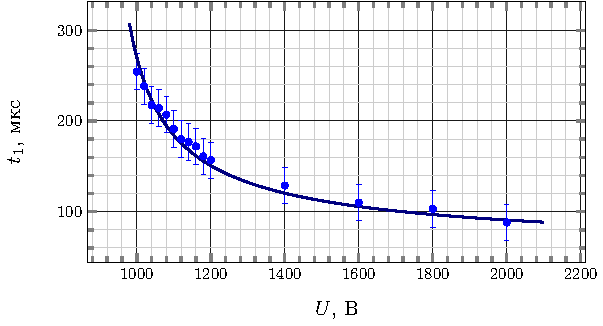
\includegraphics[scale=1.5]{fig/t1_from_u.pdf}
  \caption{Зависимость задержки генерации от накачки}
  \label{fig:figure1}
\end{figure}


\subsubsection{Длительность генерации}
\begin{figure}[H]
  \centering
  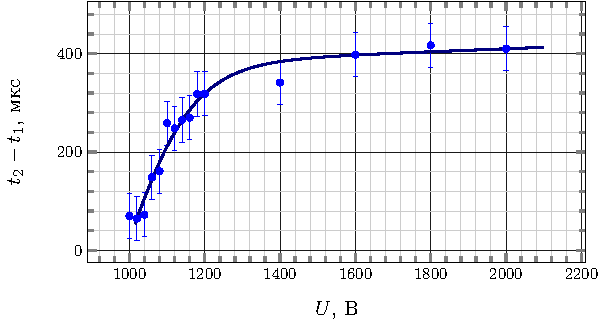
\includegraphics[scale=1.5]{fig/tau_from_u.pdf}
  \caption{Зависимость длительности генерации от накачки}
  \label{fig:figure1}
\end{figure}

\subsection{Осциллограммы излучения генерации}
\begin{figure}[H]
  \centering
  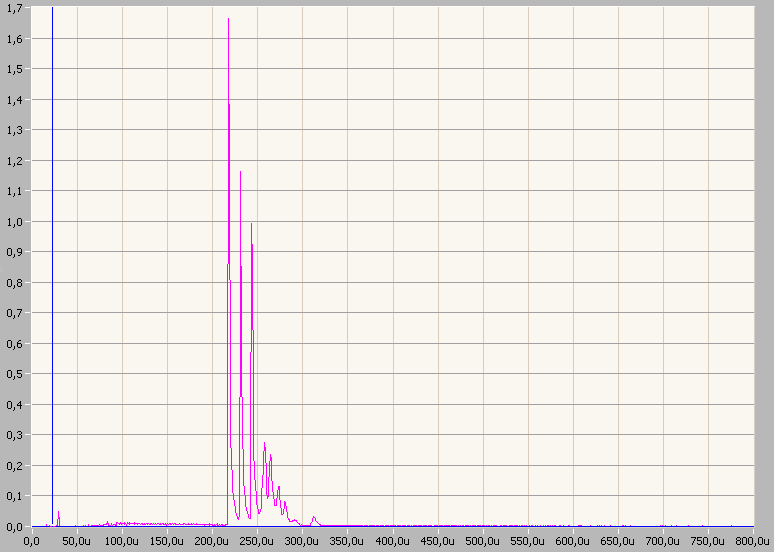
\includegraphics[width=0.8\textwidth]{png/1040Binv.png}
  \caption{Излучение генерации при $U=1040$ В}
  \label{fig:figure1}
\end{figure}
\begin{figure}[H]
  \centering
  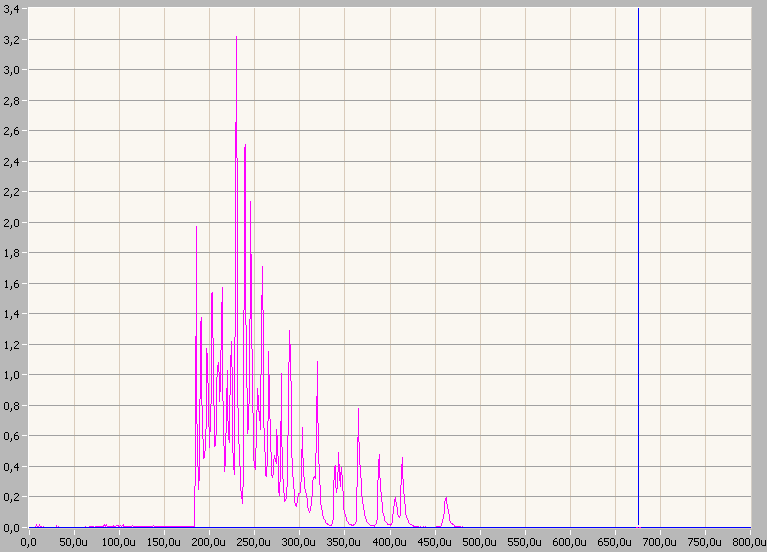
\includegraphics[width=0.8\textwidth]{png/1100Binv.png}
  \caption{Излучение генерации при $U=1100$ В}
  \label{fig:figure1}
\end{figure}
\begin{figure}[H]
  \centering
  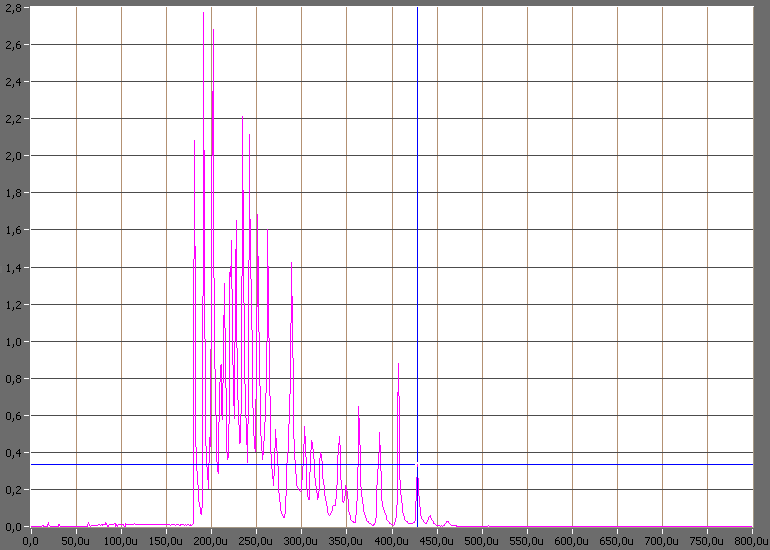
\includegraphics[width=0.8\textwidth]{png/1120Binv.png}
  \caption{Излучение генерации при $U=1120$ В}
  \label{fig:figure1}
\end{figure}

\subsection{Отдельный пичок генерации}

При напряжении накачки $U=1200$ вольт были измерены средняя\footnote{Усреднение по десяти пичкам} длительности одного пичка генерации
\begin{equation}
  \tau_1 \approx 5\text{ мкс}
\end{equation}
и средний временной интервал между пичками
\begin{equation}
  \delta t \approx 6.5\text{ мкс}.
\end{equation}
\subsection{Расчет численных величин}


\addcontentsline{toc}{section}{Заключение}
\section*{Заключение}
В настоящей работе мы 

\addcontentsline{toc}{section}{Список литературы}
\begin{thebibliography}{}

  % \bibitem{met1} Вайнштейн Л.А. Электромагнитные волны. М.: Радио и связь, 1988.
  \bibitem{met} Савикин А.П., Шарков В.В., Еремейнкин О.Н. Исследование временных характеристик твердотельного лазера на кристалле  YAG:Nd${}^{{3\texttt{+}}}$ с диодной накачкой (практикум). Н.Новгород: издательство ННГУ, 2013.

  % \bibitem{lit3} Ландау Л.Д., Лифшиц Е.М. Теория поля. М.: Физматлит, 2003.
\end{thebibliography}

\end{document}